\documentclass{article}
\usepackage[margin=1in]{geometry}
\usepackage{graphicx}
\usepackage[dvipsnames,table]{xcolor}
\usepackage[utf8]{inputenc}
\usepackage{siunitx}
\usepackage[american,siunitx]{circuitikz}
\usepackage{amsmath}
\usepackage{svg}
\usepackage{booktabs}
\usepackage{float}
\usepackage{xparse, xfp}
\usepackage{multirow}
\usepackage{tikz}
\usepackage{karnaugh-map}
\usepackage{pdfpages}
\usepackage{hyperref}
\usepackage{adjustbox}
\usepackage{listings}
\usepackage[shortlabels]{enumitem}

\definecolor{codegreen}{rgb}{0,0.6,0}
\definecolor{codegray}{rgb}{0.5,0.5,0.5}
\definecolor{codepurple}{rgb}{0.58,0,0.82}
\definecolor{backcolour}{rgb}{0.95,0.95,0.92}

\lstdefinestyle{mystyle}{
    backgroundcolor=\color{backcolour},   
    commentstyle=\color{codegreen},
    keywordstyle=\color{magenta},
    numberstyle=\tiny\color{codegray},
    stringstyle=\color{codepurple},
    basicstyle=\ttfamily\footnotesize,
    breakatwhitespace=false,         
    breaklines=true,                 
    captionpos=b,                    
    keepspaces=true,                 
    numbers=left,                    
    numbersep=5pt,                  
    showspaces=false,                
    showstringspaces=false,
    showtabs=false,                  
    tabsize=2
}
\lstset{style=mystyle}


\hypersetup{
    colorlinks=true,
    linkcolor=blue,
    filecolor=magenta,      
    urlcolor=cyan,
}
\usetikzlibrary{calc}
%\usepackage[landscape]{geometry}
\renewcommand{\thesubsection}{\thesection.\alph{subsection}}
\newcommand{\equal}{=}
\newcommand{\greyrule}{\arrayrulecolor{black!30}\midrule\arrayrulecolor{black}}
\makeatletter
\newcommand\currcoor{\the\tikz@lastxsaved,\the\tikz@lastysaved}
\makeatother
\newcolumntype{:}{@{\hskip\tabcolsep\color{black!30}\vrule\hskip\tabcolsep}}

\ExplSyntaxOn
\NewExpandableDocumentCommand \groupify { O{\,\allowbreak} m m }
  { \jakob_groupify:nnn {#1} {#2} {#3} }
\cs_new:Npn \jakob_groupify:nnn #1 #2 #3
  { \__jakob_groupify_loop:nnw { 1 } {#2} #3 \q_recursion_tail {#1} \q_recursion_stop }
\cs_new:Npn \__jakob_groupify_loop:nnw #1 #2 #3
  {
    \quark_if_recursion_tail_stop:n {#3}
    \exp_not:n {#3}
    \int_compare:nNnTF {#1} = {#2}
      { \__jakob_groupify_sep:n }
      { \exp_args:Nf \__jakob_groupify_loop:nnw { \int_eval:n { #1+1 } } }
          {#2}
  }
\cs_new:Npn \__jakob_groupify_sep:n #1 #2 \q_recursion_tail #3
  {
    \tl_if_empty:nF {#2} { \exp_not:n {#3} }
    \__jakob_groupify_loop:nnw { 1 } {#1}
    #2 \q_recursion_tail {#3}
  }
\ExplSyntaxOff

\title{ECE 4310\\Operating Systems for Embedded Application\\\,\\Homework 2}
\author{Choi Tim Antony Yung}
%\date{February 11, 2021}
\begin{document}
\maketitle

\thispagestyle{empty}
\setcounter{page}{0}

\newpage



\section{(10 pts) Explain in detail the difference between preemptive and non-preemptive scheduling.}
Preemptive scheduling can happen when a process switches from the running state to the waiting state,
when a process switches from the running state to the ready state, when a process switches from the waiting state to the ready state,
or when a process terminate; whereas nonpreemtive scheduling take place only when a process switches from the running state to the waiting state or when a process terminate.

\section{(15 pts) Consider the following processes arriving at the ready queue and dispatched to a single core CPU:}

\begin{table}[H]
  \centering
  \begin{tabular}{r|ccc}
    \toprule
    \multirow{2}{*}{PID} & Arrival & Burst & \multirow{2}{*}{Priority} \\
                         & Time    & (ms)  &                           \\
    \midrule
    10                   & 0       & 4     & 9                         \\
    11                   & 2       & 5     & 4                         \\
    12                   & 7       & 9     & 3                         \\
    13                   & 11      & 2     & 12                        \\
    14                   & 20      & 11    & 7                         \\
    15                   & 23      & 6     & 4                         \\
    \bottomrule
  \end{tabular}
\end{table}

Using the following scheduling algorithms:\\
\;\\
First-come first-served (FCFS)\\
Preemptive shortest job first (PSJF)\\
Preemptive Round-robin with 4 ms quantum\\
Priority with a priority aging of +1 every 8 ms while in the ready queue\\
\;\\
Answer the following:\\
\begin{enumerate}[(a)]
  \item Draw a Gantt chart showing the arrival time and run times for each process.
  \item Calculate the wait time for each process and average waiting time.
  \item Calculate the turnaround time for each process.
\end{enumerate}

\subsection*{FCFS}
\begin{adjustbox}{max width=\textwidth}
  \begin{tikzpicture}
    % draw horizontal line   
    \draw (0,0) -- (37,0);

    % draw vertical lines
    \foreach \x in {0,4,9,18,20,31,37}
    \draw (\x cm,10pt) -- (\x cm,-10pt);

    % draw nodes
    \draw (0,0) node[below=10pt] {\huge$ 0 $} node[above=10pt] {\huge$   $};
    \draw (4,0) node[below=10pt] {\huge$ 4 $} node[above=10pt] {\huge$   $};
    \draw (9,0) node[below=10pt] {\huge$ 9 $} node[above=10pt] {\huge$   $};
    \draw (18,0) node[below=10pt] {\huge$ 18 $} node[above=10pt] {\huge$   $};
    \draw (20,0) node[below=10pt] {\huge$ 20 $} node[above=10pt] {\huge$   $};
    \draw (31,0) node[below=10pt] {\huge$ 31 $} node[above=10pt] {\huge$   $};
    \draw (37,0) node[below=10pt] {\huge$ 37 $} node[above=10pt] {\huge$   $};

    \draw (2,0) node[below=10pt] {\huge$  $} node[above=10pt] {\huge 10};
    \draw (6.5,0) node[below=10pt] {\huge$  $} node[above=10pt] {\huge 11};
    \draw (13.5,0) node[below=10pt] {\huge$  $} node[above=10pt] {\huge 12};
    \draw (19,0) node[below=10pt] {\huge$  $} node[above=10pt] {\huge 13};
    \draw (25.5,0) node[below=10pt] {\huge$  $} node[above=10pt] {\huge 14};
    \draw (34,0) node[below=10pt] {\huge$  $} node[above=10pt] {\huge 15};

  \end{tikzpicture}
\end{adjustbox}
\begin{table}[H]
  \centering
  \begin{tabular}{r|rr}
    \toprule
    \multirow{2}{*}{PID} & Wait      & Turnaround \\
            & Time      & Time       \\
    \midrule
    10      & $ 0-0 =0$ & $ 4-0 =4 $ \\
    11      & $ 4-2 =2$ & $ 9-2 =7 $ \\
    12      & $ 9-7 =2$ & $18-7 =11$ \\
    13      & $18-11=7$ & $20-11=9 $ \\
    14      & $20-20=0$ & $31-20=11$ \\
    15      & $31-23=8$ & $37-23=14$ \\
    \bottomrule
  \end{tabular}
\end{table}
$\text{Average wait time} = \frac{1}{6}(0+2+2+7+0+8)\approx3.17$

\subsection*{PSJF}
\begin{adjustbox}{max width=\textwidth}
  \begin{tikzpicture}
    % draw horizontal line   
    \draw (0,0) -- (37,0);

    % draw vertical lines
    \foreach \x in {0,4,9,11,13,20,23,29,37}
    \draw (\x cm,10pt) -- (\x cm,-10pt);

    % draw nodes
    \draw (0,0) node[below=10pt] {\huge$ 0 $} node[above=10pt] {\huge$   $};
    \draw (4,0) node[below=10pt] {\huge$ 4 $} node[above=10pt] {\huge$   $};
    \draw (9,0) node[below=10pt] {\huge$ 9 $} node[above=10pt] {\huge$   $};
    \draw (11,0) node[below=10pt] {\huge$ 11 $} node[above=10pt] {\huge$   $};
    \draw (13,0) node[below=10pt] {\huge$ 13 $} node[above=10pt] {\huge$   $};
    \draw (20,0) node[below=10pt] {\huge$ 20 $} node[above=10pt] {\huge$   $};
    \draw (23,0) node[below=10pt] {\huge$ 23 $} node[above=10pt] {\huge$   $};
    \draw (29,0) node[below=10pt] {\huge$ 29 $} node[above=10pt] {\huge$   $};
    \draw (37,0) node[below=10pt] {\huge$ 37 $} node[above=10pt] {\huge$   $};

    \draw (2,0) node[below=10pt] {\huge$  $} node[above=10pt] {\huge 10};
    \draw (6.5,0) node[below=10pt] {\huge$  $} node[above=10pt] {\huge 11};
    \draw (10,0) node[below=10pt] {\huge$  $} node[above=10pt] {\huge 12};
    \draw (12,0) node[below=10pt] {\huge$  $} node[above=10pt] {\huge 13};
    \draw (16.5,0) node[below=10pt] {\huge$  $} node[above=10pt] {\huge 12};
    \draw (21.5,0) node[below=10pt] {\huge$  $} node[above=10pt] {\huge 14};
    \draw (26,0) node[below=10pt] {\huge$  $} node[above=10pt] {\huge 15};
    \draw (33,0) node[below=10pt] {\huge$  $} node[above=10pt] {\huge 14};

  \end{tikzpicture}
\end{adjustbox}
\begin{table}[H]
  \centering
  \begin{tabular}{r|rr}
    \toprule
    \multirow{2}{*}{PID} & Wait      & Turnaround \\
            & Time      & Time       \\
    \midrule
    10      & $ 0-0 =0$ & $ 4-0 =4 $ \\
    11      & $ 4-2 =2$ & $ 9-2 =7 $ \\
    12      & $ (13-11)+(9-7) =4$ & $20-7 =13$ \\
    13      & $11-11=0$ & $13-11=2 $ \\
    14      & $(29-23)+(20-20)=6$ & $37-20=17$ \\
    15      & $23-23=0$ & $29-23=6$ \\
    \bottomrule
  \end{tabular}
\end{table}
$\text{Average wait time} = \frac{1}{6}(0+2+4+0+6+0)=2$

\subsection*{Preemptive Round-robin with 4 ms quantum}
\begin{adjustbox}{max width=\textwidth}
  \begin{tikzpicture}
    % draw horizontal line   
    \draw (0,0) -- (37,0);

    % draw vertical lines
    \foreach \x in {0,4,8,12,14,15,19,20,24,28,32,34,37}
    \draw (\x cm,10pt) -- (\x cm,-10pt);

    % draw nodes
    \draw (0,0) node[below=10pt] {\huge$ 0 $} node[above=10pt] {\huge$   $};
    \draw (4,0) node[below=10pt] {\huge$ 4 $} node[above=10pt] {\huge$   $};
    \draw (8,0) node[below=10pt] {\huge$ 8 $} node[above=10pt] {\huge$   $};
    \draw (12,0) node[below=10pt] {\huge$ 12 $} node[above=10pt] {\huge$   $};
    \draw (14,0) node[below=10pt] {\huge$ 14 $} node[above=10pt] {\huge$   $};
    \draw (15,0) node[below=10pt] {\huge$ 15 $} node[above=10pt] {\huge$   $};
    \draw (19,0) node[below=10pt] {\huge$ 19 $} node[above=10pt] {\huge$   $};
    \draw (20,0) node[below=10pt] {\huge$ 20 $} node[above=10pt] {\huge$   $};
    \draw (24,0) node[below=10pt] {\huge$ 24 $} node[above=10pt] {\huge$   $};
    \draw (28,0) node[below=10pt] {\huge$ 28 $} node[above=10pt] {\huge$   $};
    \draw (32,0) node[below=10pt] {\huge$ 32 $} node[above=10pt] {\huge$   $};
    \draw (34,0) node[below=10pt] {\huge$ 34 $} node[above=10pt] {\huge$   $};
    \draw (37,0) node[below=10pt] {\huge$ 37 $} node[above=10pt] {\huge$   $};

    \draw (2,0) node[below=10pt] {\huge$  $} node[above=10pt] {\huge 10};
    \draw (6,0) node[below=10pt] {\huge$  $} node[above=10pt] {\huge 11};
    \draw (10,0) node[below=10pt] {\huge$  $} node[above=10pt] {\huge 12};
    \draw (13,0) node[below=10pt] {\huge$  $} node[above=10pt] {\huge 13};
    \draw (14.5,0) node[below=10pt] {\huge$  $} node[above=10pt] {\huge 11};
    \draw (17,0) node[below=10pt] {\huge$  $} node[above=10pt] {\huge 12};
    \draw (19.5,0) node[below=10pt] {\huge$  $} node[above=10pt] {\huge 12};
    \draw (22,0) node[below=10pt] {\huge$  $} node[above=10pt] {\huge 14};
    \draw (26,0) node[below=10pt] {\huge$  $} node[above=10pt] {\huge 15};
    \draw (30,0) node[below=10pt] {\huge$  $} node[above=10pt] {\huge 14};
    \draw (33,0) node[below=10pt] {\huge$  $} node[above=10pt] {\huge 15};
    \draw (35.5,0) node[below=10pt] {\huge$  $} node[above=10pt] {\huge 14};

  \end{tikzpicture}
\end{adjustbox}
\begin{table}[H]
  \centering
  \begin{tabular}{r|rr}
    \toprule
    \multirow{2}{*}{PID} & Wait      & Turnaround \\
            & Time      & Time       \\
    \midrule
    10      & $ 0-0 =0$ & $ 4-0 =4 $ \\
    11      & $ (14-8)+(4-2) =8$ & $ 15-2 =13 $ \\
    12      & $ (15-12)+(8-7) =4$ & $20-7 =13$ \\
    13      & $12-11=1$ & $14-11=3 $ \\
    14      & $(34-32)+(28-24)+(20-20)=6$ & $37-20=17$ \\
    15      & $(32-28)+(24-23)=5$ & $34-23=11$ \\
    \bottomrule
  \end{tabular}
\end{table}
$\text{Average wait time} = \frac{1}{6}(0+8+4+1+6+5)\approx3.7$

\subsection*{Priority with a priority aging of +1 every 8 ms while in the ready queue}
\begin{adjustbox}{max width=\textwidth}
  \begin{tikzpicture}
    % draw horizontal line   
    \draw (0,0) -- (37,0);

    % draw vertical lines
    \foreach \x in {0,2,7,16,18,20,23,29,37}
    \draw (\x cm,10pt) -- (\x cm,-10pt);

    % draw nodes
    \draw (0,0) node[below=10pt] {\huge$ 0 $} node[above=10pt] {\huge$   $};
    \draw (2,0) node[below=10pt] {\huge$ 2 $} node[above=10pt] {\huge$   $};
    \draw (7,0) node[below=10pt] {\huge$ 7 $} node[above=10pt] {\huge$   $};
    \draw (16,0) node[below=10pt] {\huge$ 16 $} node[above=10pt] {\huge$   $};
    \draw (18,0) node[below=10pt] {\huge$ 18 $} node[above=10pt] {\huge$   $};
    \draw (20,0) node[below=10pt] {\huge$ 20 $} node[above=10pt] {\huge$   $};
    \draw (23,0) node[below=10pt] {\huge$ 23 $} node[above=10pt] {\huge$   $};
    \draw (29,0) node[below=10pt] {\huge$ 29 $} node[above=10pt] {\huge$   $};
    \draw (37,0) node[below=10pt] {\huge$ 37 $} node[above=10pt] {\huge$   $};

    \draw (1,0) node[below=10pt] {\huge$  $} node[above=10pt] {\huge 10};
    \draw (4.5,0) node[below=10pt] {\huge$  $} node[above=10pt] {\huge 11};
    \draw (11.5,0) node[below=10pt] {\huge$  $} node[above=10pt] {\huge 12};
    \draw (17,0) node[below=10pt] {\huge$  $} node[above=10pt] {\huge 10};
    \draw (19,0) node[below=10pt] {\huge$  $} node[above=10pt] {\huge 13};
    \draw (21.5,0) node[below=10pt] {\huge$  $} node[above=10pt] {\huge 14};
    \draw (26,0) node[below=10pt] {\huge$  $} node[above=10pt] {\huge 15};
    \draw (33,0) node[below=10pt] {\huge$  $} node[above=10pt] {\huge 14};

  \end{tikzpicture}
\end{adjustbox}
\begin{table}[H]
  \centering
  \begin{tabular}{r|rr}
    \toprule
    \multirow{2}{*}{PID} & Wait      & Turnaround \\
            & Time      & Time       \\
    \midrule
    10      & $ (16-2)+(0-0) =14$ & $ 18-0 =18$ \\
    11      & $ 2-2 =0$ & $ 7-2 =5 $ \\
    12      & $ 7-7 =0$ & $16-7 =9$ \\
    13      & $18-11=7$ & $20-11=9 $ \\
    14      & $(29-23)+(20-20)=6$ & $37-20=17$ \\
    15      & $23-23=0$ & $29-23=6$ \\
    \bottomrule
  \end{tabular}
\end{table}
$\text{Average wait time} = \frac{1}{6}(14+0+0+7+6+0)\approx4.5$

\section{(10 pts) What is an atomic operation? Provide at least one detailed example of an atomic operation.}
An atomic operation is an operation that must be executed fully uninterrupted.
An example is \texttt{acquire()} for mutex lock. \texttt{acquire()} have two part: the busy wait part and the set unavailable part.
The process will constantly check for availability of mutex lock and once it become available, it must set it to unavailable before
 it is acquired by other process. Therefore, it must set the lock unavailable immediately after the wait ends.

\section{(15 pts) Recall the various deadlock detection and prevention algorithms we’ve discussed in class and consider the following snapshot of a system with five processes (P10, P11, P12, P13, P14) and four resources (R1, R2, R3, R4).  R1, R2, R3, and R4 have a total of 4, 7, 2, and 11 resources, respectively.  There are no current outstanding queued unsatisfied requests.}
\begin{table}[H]
  \begin{minipage}{.5\textwidth}
    \centering
  \caption{Allocation}
  \begin{tabular}{c|cccc}
    \toprule
    PID & R1 & R2 & R3 & R4\\
    \midrule
    10      & 1 & 0 & 1 & 8 \\
    11      & 0 & 2 & 0 & 1 \\
    12      & 2 & 0 & 0 & 0 \\
    13      & 0 & 1 & 1 & 1 \\
    14      & 1 & 3 & 0 & 1 \\
    \bottomrule
  \end{tabular}
  \label{tbl:4_1}
  \end{minipage}
  \begin{minipage}{.5\textwidth}
    \centering
  \caption{Max Need}
  \begin{tabular}{c|cccc}
    \toprule
    PID & R1 & R2 & R3 & R4\\
    \midrule
    10      & 3 & 1 & 2 & 8 \\
    11      & 0 & 6 & 2 & 5 \\
    12      & 2 & 1 & 2 & 10 \\
    13      & 1 & 7 & 2 & 3 \\
    14      & 4 & 5 & 2 & 4 \\
    \bottomrule
  \end{tabular}
  \label{tbl:4_2}
  \end{minipage}
\end{table}

Is the system currently in a safe or unsafe state?  If safe, provide the process execution order.

\begin{table}[H]
    \centering
  \caption{Need}
  \begin{tabular}{c|cccc}
    \toprule
    PID & R1 & R2 & R3 & R4\\
    \midrule
    10      & 2 & 1 & 1 & 0 \\
    11      & 0 & 4 & 2 & 4 \\
    12      & 0 & 1 & 2 & 10\\
    13      & 1 & 6 & 1 & 2 \\
    14      & 3 & 2 & 2 & 3 \\
    \bottomrule
  \end{tabular}
  \label{tbl:4_3}
\end{table}

$Available = (4,7,2,11)-(1,0,1,8)-(0,2,0,1)-(2,0,0,0)-(0,1,1,1)-(1,3,0,1)=(0,1,0,0)$\\
Initialize: $Work = Available$, $Finish = (False, False, False, False, False)$\\
Check P10: $Finish[10] = False$, $Need_{10} = (2,1,1,0) > (0,1,0,0) = Work$\\
Check P11: $Finish[11] = False$, $Need_{11} = (0,4,2,4) > (0,1,0,0) = Work$\\
Check P12: $Finish[12] = False$, $Need_{12} = (0,1,2,10) > (0,1,0,0) = Work$\\
Check P13: $Finish[13] = False$, $Need_{13} = (1,6,1,2) > (0,1,0,0) = Work$\\
Check P14: $Finish[14] = False$, $Need_{14} = (3,2,2,3) > (0,1,0,0) = Work$\\
Not enough resources to finish any process, system in an unsafe state.

\end{document}